\ylDisplay{Rattamatk} % Ülesande nimi
{Ardi Loot} % Autor
{lahtine} % Voor
{2017} % Aasta
{G 5} % Ülesande nr.
{4} % Raskustase
{
% Teema: Gaasid
\ifStatement
Juku on rattamatkal ning soovib ratta tagumist rehvi natuke rohkem
täis pumbata. Et oleks lihtsam, kulutab Juku palju vaeva ja pakib
raske matkavarustuse pakiraamilt maha ja keerab ratta tagurpidi (rattad
taeva poole). Hinnake, mitu protsenti vähem jõudu peab ta pumpamisel
rakendama võrreldes olukorraga, kui tagumine ratas on koormatud?

\begin{wrapfigure}[5]{r}{0.4\linewidth}
	\vspace{-15pt}
	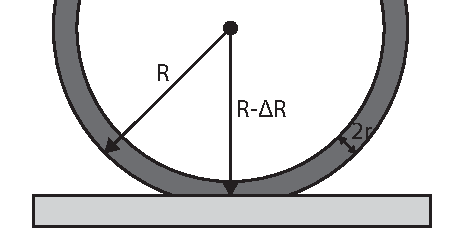
\includegraphics[width=\linewidth]{2017-lahg-05-fig_rattakumm.pdf}
\end{wrapfigure}

Ratta raadius $R=\SI{33.0}{cm},$ rehvi raadius $r=\SI{2.5}{cm},$
tagumisele rattale toetuv mass (ratas koos matkavarustusega) $m=\SI{30}{kg},$
koormatud rehvi rõhk $p=\SI{150}{kPa}$ (mõõdetud õhurõhu suhtes), õhurõhk $p_{0}=\SI{100}{kPa}$
ja raskuskiirendus $g=\SI{9.8}{m/s^{2}}.$ 

\textit{Vihje}. Koormamata rattarehvi ruumala on antud valemiga $V=2\pi^{2}\left(R-r\right)r^{2}$
ning see väheneb koormamisel $\Delta V\approx S\cdot\Delta R/2$ võrra,
kus $S\approx2\pi\Delta R\sqrt{Rr}$ on rehvi kokkupuutepinna suurus
maaga ja $\Delta R\ll r$ on rehvi deformatsiooni ulatus (vt joonist).
\fi


\ifHint
On selge, et rehvi pumpamisel on rakendatav jõud võrdeline rehvis oleva rõhuga (õhurõhu suhtes). Rakendades jõudude tasakaalutingimust rehvi kokkupuutepinnale maaga, on võimalik leida kokkupuutepinna pindala, millest saab omakorda avaldada rehvi deformatsiooni ning rattarehvi ruumala muudu. Rattarehvi ruumala muudust tingitud rehvi siserõhu muutu on võimalik avaldada ideaalse gaasivõrrandiga.
\fi


\ifSolution
Koormatud rehvi kokkupuutepinnale maaga mõjuvad ühelt poolt rehvi sees oleva suruõhu poolt jõud $\left(p_{0}+p\right)S$ ning teiselt
poolt õhurõhu poolt tekitatud jõud $p_{0}S$ ja maapinna reaktsioonijõud $mg$. Nende jõudude tasakaalutingimus annab meile võrrandi $\left(p_{0}+p\right)S=p_{0}S+mg.$ Kasutades avaldist rehvi kokkupuutepinna suuruse $S\approx2\pi\Delta R\sqrt{Rr}$ sõltuvusest deformatsioonist $\Delta R$, saame leida, et rehv on deformeeritud

\begin{equation}
\Delta R=\frac{mg}{2\pi p\sqrt{Rr}}\approx\SI{3.4}{mm}
\end{equation}

\noindent võrra.

Rehvilt koormuse eemaldamise tulemusena suureneb selle ruumala $\Delta V\approx S\cdot\Delta R/2\approx\SI{3.4}{cm^{3}}$ võrra ja seetõttu väheneb suruõhu rõhk rehvis $\Delta p$ võrra. Kasutades ideaalse gaasi võrrandit, saame tingimuse $\left(p_{0}+p\right)\left(V-\Delta V\right)=\left(p_{0}+p-\Delta p\right)V$
ja selle lahendamisel

\begin{equation}
\Delta p=\left(p_{0}+p\right)\frac{\Delta V}{V}\approx\SI{224}{Pa}.
\end{equation}

On selge, et rehvi pumpamisel on rakendatav jõud võrdeline rehvis oleva rõhuga (õhurõhu suhtes) ja seega peab ta rakendama vaid 
\[
\frac{\Delta p}{p}=\frac{\left(p+p_{0}\right)m^{2}g^{2}}{8\pi^{3}p^{3}\left(R-r\right)r^{2}\sqrt{Rr}}\approx\SI{0.15}{\percent}
\]
võrra vähem jõudu võrreldes olukorraga, kui rehv on koormatud.
\fi


\ifEngStatement
% Problem name: Bicycle hike
\begin{wrapfigure}[6]{r}{0.4\linewidth}
	\vspace{-15pt}
	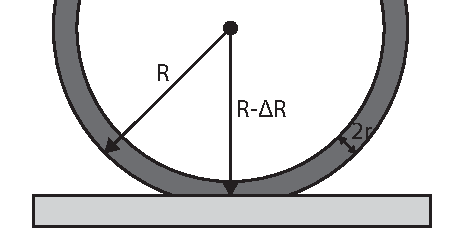
\includegraphics[width=5cm]{2017-lahg-05-fig_rattakumm}
\end{wrapfigure}
Juku is on a bicycle hike and wants to pump a little more air into his bike’s rear wheel. To make things easier, Juku packs his heavy hike equipment off the rack and turns the bike upside down (wheels are directed towards the sky). Estimate by how many percent smaller force he needs to apply while pumping as compared to the situation where the equipment was still on. The radius of the wheel is $R=\SI{33.0}{cm}$, radius of the tire $r=\SI{2.5}{cm}$, the mass resting on the rear wheel (the wheel together with the hike equipment) $m=\SI{30}{kg}$, the gauge pressure in the wheel under the load $p=\SI{150}{kPa}$, air pressure $p_{0}=\SI{100}{kPa}$ and gravitational acceleration $g=\SI{9.8}{m/s^{2}}$.\\
\emph{Hint.} The mass of the wheel without the load is given by an equation $V=2\pi^{2}\left(R-r\right)r^{2}$ and with loading it decreases by $\Delta V\approx S\cdot\Delta R/2$, where $S\approx2\pi\Delta R\sqrt{Rr}$ is the area of contact between the tire and the ground and $\Delta R\ll r$ is the range of tire’s deformation (see figure).
\fi


\ifEngHint
It is clear that when pumping the tire the force applied is proportional to the pressure inside the tire (with respect to the air pressure). Using the equilibrium condition of the forces on the touching surface between the tire and the ground it is possible to find the area of the touching surface from which in turn it is possible to express the deformation of the tire and the volume change of the bike tire. The change of the tire's inner pressure caused by the volume change of the bike tire change is possible to find with the ideal gas law.
\fi


\ifEngSolution
The contact surface of the weighted tire and the ground is from one side applied with the force $\left(p_{0}+p\right)S$ caused by the compressed air inside the tire and from the other side with the force $p_{0}S$ caused by the air pressure and the ground’s normal force of the ground $mg$. The balance of these forces give us the equation $\left(p_{0}+p\right)S=p_{0}S+mg.$. Using this for the tire’s contact surface size $S\approx2\pi\Delta R\sqrt{Rr}$ dependence on deformation $\Delta R$ we can find that the tire is deformed by 
\begin{equation}
\Delta R=\frac{mg}{2\pi p\sqrt{Rr}}\approx\SI{3.4}{mm}
\end{equation} 
If the weight is removed from the tire then the tire’s velocity increases by $\Delta V\approx S\cdot\Delta R/2\approx\SI{3.4}{cm^{3}}$ and because of this the compressed air pressure in the tire decreases by $\Delta p$. Using the ideal gas law we get the condition $\left(p_{0}+p\right)\left(V-\Delta V\right)=\left(p_{0}+p-\Delta p\right)V$ and solving this
\begin{equation}
\Delta p=\left(p_{0}+p\right)\frac{\Delta V}{V}\approx\SI{224}{Pa}.
\end{equation} 
It is clear that the force applied while pumping the tire is proportional to the pressure inside the tire (with respect to the air pressure) and therefore Juku only has to apply 
\[
\frac{\Delta p}{p}=\frac{\left(p+p_{0}\right)m^{2}g^{2}}{8\pi^{3}p^{3}\left(R-r\right)r^{2}\sqrt{Rr}}\approx\SI{0.15}{\percent}
\] 
less force compared to the situation when the tire has a weight on it.
\fi
}